\section{MIMO}
\subsection{MIMO概述}
多输入多输出MIMO(Multiple-Input Multiple-Output),指在发射端和接收端分别使用多个天线传送和接收信号,从而改善通信质量。通过多个天线实现多发多收,在频谱资源和天线发射功率不变的情况下,充分利用空间资源,成倍地提高系统信道容量,增加了频谱利用率。根据网上查阅到的资料,MIMO已被用于802.11n标准,并且被用于改进802.11 a/b/g网络的性能。\par
一个典型性的MIMO系统如图\ref{MIMO}所示。发射端通过空间——时间映射(空时映射)将数据信号映射到多根天线上,接收端将各根天线接收到的信号进行空时译码,恢复出发射端发送的数据信号。
\begin{figure}[H]
	\centering
	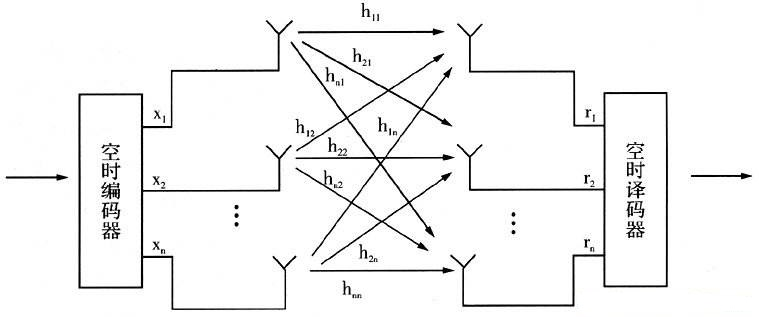
\includegraphics[scale=2]{MIMOfig1}
	\caption{MIMO系统结构图.}
	\label{MIMO}
\end{figure}

无线电发送的信号被反射时,会产生多份信号,每份信号都是一个空间流。单输入单输出(SISO)系统一次只能发送或接收一个空间流。相比于SISO,MIMO主要有以下两大优点:\\
\textbf{1 }提高了信道容量。这是因为MIMO允许多个天线同时发送和接收多个空间流,极大地提高了信号传输的效率。MIMO技术的应用,使空间成为一种可以用于提高性能的资源,并能够增加无线系统的覆盖范围。\\
\textbf{2 }提高了信道的可靠性。利用MIMO信道提供的空间复用增益及空间分集增益,可以利用多天线来抑制信道衰落。多天线系统的应用,使得并行数据流可以同时传送,可以显著克服信道的衰落,降低误码率。\par
(以上资料部分来自相关教材和互联网)

\subsection{数学模型}
MIMO系统中的输入输出关系可描述为
\[
r=Hx+n
\]
其中$x=[x_1,x_2,\dots,x_{n_T}]$为多维输入信号矢量构成的矩阵,$r=[r_1,r_2,\dots,r_{n_R}]$为接受信号构成的矩阵,$H$为信道转移矩阵,$n$为加性高斯白噪声.



